\documentclass[oneside,openright,uplatex]{jsbook} % oneside: 章ごとに改ページ.twoside: 章の初めが右側となるように改ページ.

% jsbookで余白が広すぎるのを直す
% 参照 https://oku.edu.mie-u.ac.jp/~okumura/jsclasses/
\setlength{\textwidth}{\fullwidth}
\setlength{\evensidemargin}{\oddsidemargin}

% OTF フォントを使えるようにし、複数のウェイトも使用可能にする。
% これがないと、Mac のヒラギノ環境で使われる角ゴが太すぎてみっともない。
\usepackage[deluxe]{otf}

% OT1→T1に変更し、ウムラウトなどを PDF 出力で合成文字ではなくす
\usepackage[T1]{fontenc}

% uplatex の場合に必要な処理 
\usepackage[utf8]{inputenc} % エンコーディングが UTF8 であることを明示する。
\usepackage[prefernoncjk]{pxcjkcat} % アクセントつきラテン文字を欧文扱いにする

% Helvetica と Times を sf と rm のそれぞれで使う。
% default だとバランスが悪いので、日本語に合わせて文字の大きさを調整する。
\usepackage[scaled=1.05,helvratio=0.95]{newtxtext}

% 画像の取り扱いに必要
\usepackage[dvipdfmx]{graphicx}

% 表でセルを複数列で結合する
\usepackage{multicol}

% 数式の機能を拡張
\usepackage{amsmath}

% citep や citet を有効にする
\usepackage{natbib}

% (Okumura, 2009) などを (Okumura 2009) とする
\setcitestyle{aysep={}}

% subfigure 環境で、(a)、(b) などの番号を左上に表示する。宇宙系の分野ではこれが一般的なはず。
\usepackage[nooneline]{subfigure}
\subfiguretopcaptrue

% 行番号を表示する。添削時のみに使い、事務提出版ではコメントアウトする
%\usepackage{lineno}
%\linenumbers

% PDF 内で外部リンクや文書内リンクを生成したい場合に使う(好みによる)
% \usepackage[dvipdfmx]{hyperref}

% newcommand を使うことで、繰り返し使う長ったらしい入力を簡単にすることができる
\makeatletter
\newcommand{\ion}[2]{#1$\;${\small\rmfamily\@Roman{#2}}\relax}%
\makeatother
\newcommand{\HI}{\mbox{\ion{H}{1}}} % 中性原子ガス(HI 領域)の例
\newcommand{\bs}{\symbol{92}} % backslash

%%%%%%%%%%%%%%%%%%%%%%%%%%%%%%%%%%%%%%%%%%%%%%%%%%%%%%%%%%%%%%%%%%%%%%%%%%%%%%%%%%%%%%%%%%%%%%%%%%%%%%%%%%%%%%%%%%%%%%%%%%%%%%

% 図を通し番号にする: http://rexpit.blog29.fc2.com/blog-entry-99.html
\usepackage{remreset}	% removefromreset に使う
\makeatletter
	\@removefromreset{figure}{chapter}
	\def\thefigure{\arabic{figure}}

	\@removefromreset{table}{chapter}
	\def\thetable{\arabic{table}}

	\@removefromreset{equation}{chapter}
	\def\theequation{\arabic{equation}}
\makeatother

\usepackage{comment} % \begin{comment} \end{comment}
\usepackage{color}   % {\color{red}メモ}

\usepackage{natbib} % citep や citet を有効にする
\bibpunct[:]{[}{]}{,}{a}{}{,} % 括弧を () -> [] へ変更
%\usepackage[numbers]{natbib} % citep や citet を有効にする
%\bibpunct[:]{(}{)}{,}{a}{}{,}

\usepackage[]{multicol}         % 段組み % \begin{multicols}{2}%2段組み開始 ~ \end{multicols}%2段組み終了

\usepackage{wrapfig}            % 図の回り込みを許す.\begin{figure}~\end{figure} -> \begin{wrapfigure}{r}{90mm}~\end{wrapfigure} へ置き換え
                                % 直後の文が制御記号だと,回り込みに失敗し,文字が図下に重なるので,制御記号の直前に ''\noindent \ \ '' を挿入して回避する.

%%%%%%%%%%%%%%%%%%%%%%%%%%%%%%%%%%%%%%%%%%%%%%%%%%%%%%%%%%%%%%%%%%%%%%%%%%%%%%%%%%%%%%%%%%%%%%%%%%%%%%%%%%%%%%%%%%%%%%%%%%%%%%

\begin{document}

\begin{titlepage}


\vspace*{120truept}
\begin{center}
  \huge{学 \ 士 \ 論 \ 文 / \ 修 \ 士 \ 論 \ 文}\\
  \vspace{30truept}
  \huge{タイトルが\\長い場合はいい感じに改行}\\ % title
\vspace{100truept}
\LARGE{xx大学大学院xxxx研究科}\\
\LARGE{xxxx専攻xxxx分野xx研究室}\\
\LARGE{苗字 名前}\\
\end{center}

%\newpage
%\thispagestyle{empty} % このページのページ番号を表示しない.
%\ % add emptypage

\end{titlepage}
 % 表紙
\thispagestyle{empty} % ページ番号を表示しない.

% レイアウトを他の章のはじめのページと揃える.
 \\
\\
\\
\\
\noindent{\Huge \sf Abstract/要旨}\\
\\
\\
\\

Abstractを書きます.




\frontmatter     % make page number roman
\tableofcontents % 目次
%\listoffigures  % 図目次
%\listoftables   % 表目次

\mainmatter      % make page number arabic
\chapter{Introduction/序論}
\label{chap_Introduction}

\section{Introduction}
イントロダクション.

\section{Review}
先行研究.

\section{Purpose}
研究目的.


\chapter{Device}
\label{chap_Device}

実験装置/観測装置について説明する.タイトルは実験/観測装置の名称などにする.



\chapter{ガンマ線天文学とCTA計画}
\label{chap_review}

この章では、自分の研究に関連する分野の歴史や現状について説明したり、研究を展開する上で重要となる知識の解説を行います。ここで使用している見出し「ガンマ線天文学…」はあくまで例ですが、もしCherekov Telescope Array(CTA)計画\footnote{省略語は必ず正式名称を先に書き、省略系は丸括弧に入れます。省略語はあくまで「以降このように略す」という用途だからです。また、日本語文章中で使う丸括弧は()ではなく()です。}に携わる院生の書く修士論文であれば、ガンマ線天文学や宇宙線物理学全般について、現行望遠鏡とガンマ線観測の原理について、またCTA計画についての記述がこの章では期待されます。

場合によっては「序論」と合体させても良いですが、本章は比較的長くなり結論に直結しない情報もたくさん出てくるため、独立した章である方が読者は読みやすいでしょう。

またこの章が長くなるときには、例えば「ガンマ線天文学」と「CTA計画」のように、2つの章に分割するというのも良いと思います。

\chapter{自分の研究本体を述べるところ}
ここは自分のやった研究を述べる章です。実際の中身に合わせて章を複数立てにする場合もあると思います。「議論」の章を別に分ける場合は、この章では得られた結果までを記述し、その結果に対する議論は「議論」の章に回すのが良いでしょう。

修士論文で大切なことは、章~\ref{chap_intro}や章~\ref{chap_review}で述べた伏線(研究の目的と動機)を回収するべく、きちんと研究内容を順序立てて書き、また自分の貢献を明確にすることです。論文全体で論理展開がきちんとしていれば良いので、必ずしも実際に行った実験などの時系列でこの章を書き進める必要はありません。また修士論文としての完成度が大切ですので、修士論文のテーマに直接関係のない自分のやったことを無理に混ぜる必要もありません。

本文書では、\LaTeX{}の使い方を以下説明します。\textbf{\textsf{ここでの表示例は本PDFを読むだけではどのような\LaTeX{}コードに対応しているか分かりませんので、\texttt{main.tex}や\texttt{WhatYouDid.tex}の中身を参照してください。}}

このPDF文書中に\texttt{command}のような書体で記載されているものは、\LaTeX{}ソース中で実際に入力するコマンドやファイル名を示しています。

\section{節の使い方}
\texttt{\bs{}section}や\texttt{\bs{}subsection}を使うと「節」(section)と呼ばれる構造を作ることができます。長い章を分割して論理展開を分かりやすくする目的で使います。

文中で節を参照するときは、\texttt{section}であっても\texttt{subsection}であっても「節」と呼び、「\ref{sec_figure}~節」や「第\ref{sec_figure}~節」のように書きます(\texttt{ref}コマンドの使用は次節参照)。章を参照するときは「\ref{chap_review}~章」や「第\ref{chap_review}~章」とします。

\section{図の使い方}
\label{sec_figure} % このようにラベルをつけることで、\refコマンドで節や図の番号を参照できます。

論文中に図を入れるときは、\texttt{figure}環境を使用します。画像形式は図~\ref{fig_CTA}のようなJPEG(主に写真などに最適)やPNG(色数の少ない画像に最適)に加え、図~\ref{fig_histogram}のようにPDF(グラフなどに最適)も使うことができます。実際の使い方は、この\LaTeX{}のコードを読んでください。\textsf{\textbf{EPS形式はいまどき誰も使いません。古い\LaTeX{}の本や年寄りに騙されないでください。}}

\begin{figure} % 特に強い理由がない限り、[htbp]のような指定はしないでください。
  \centering
  % 図の横幅をちょうど良い具合に自分で調整します。
  % 図中の文字を読めないような大きさにはしないでください。
  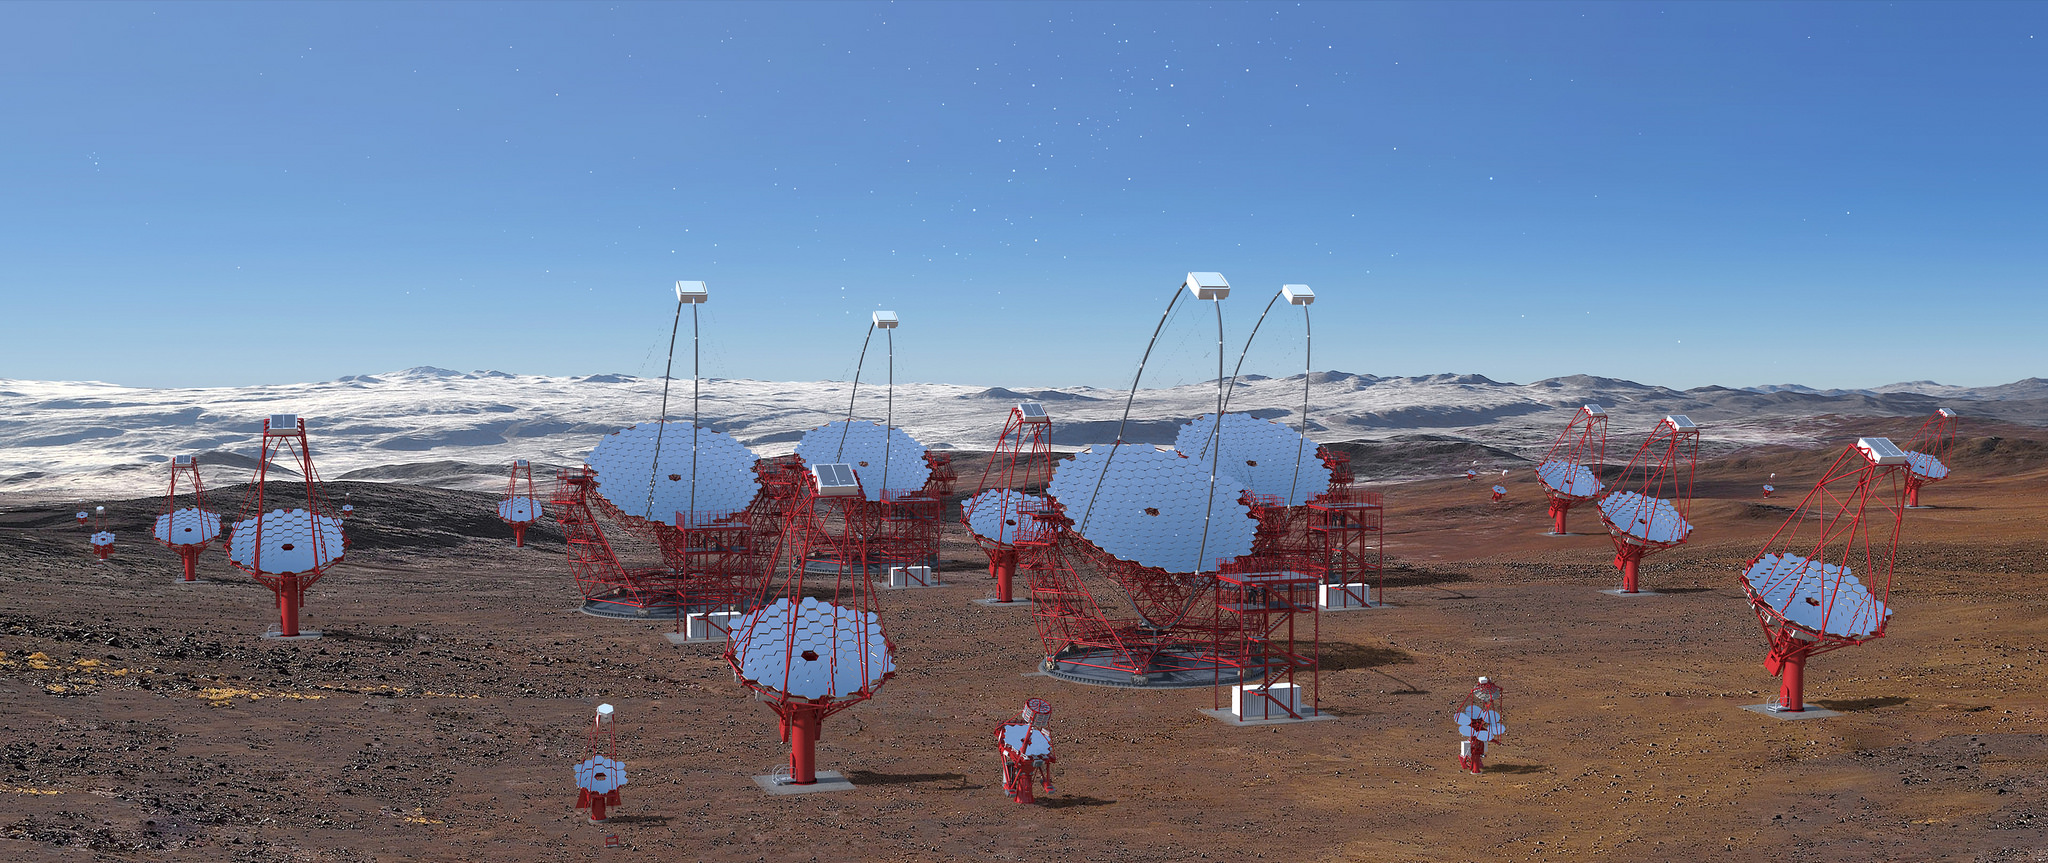
\includegraphics[width=14cm]{fig/CTA.jpg}
  % 図の説明が長い場合、[]で囲むことで短い図の説明を目次のみに表示できます。
  \caption[CTAの完成想像図]{CTAの完成想像図(画像提供:CTA Consortium)。JPEG(ビットマップ画像)なので、出力PDFで拡大するとドットが見えます。}
  % これで本文中から参照できます。
  \label{fig_CTA}
\end{figure}

\begin{figure}
  \centering
  % PDFも使えます。
  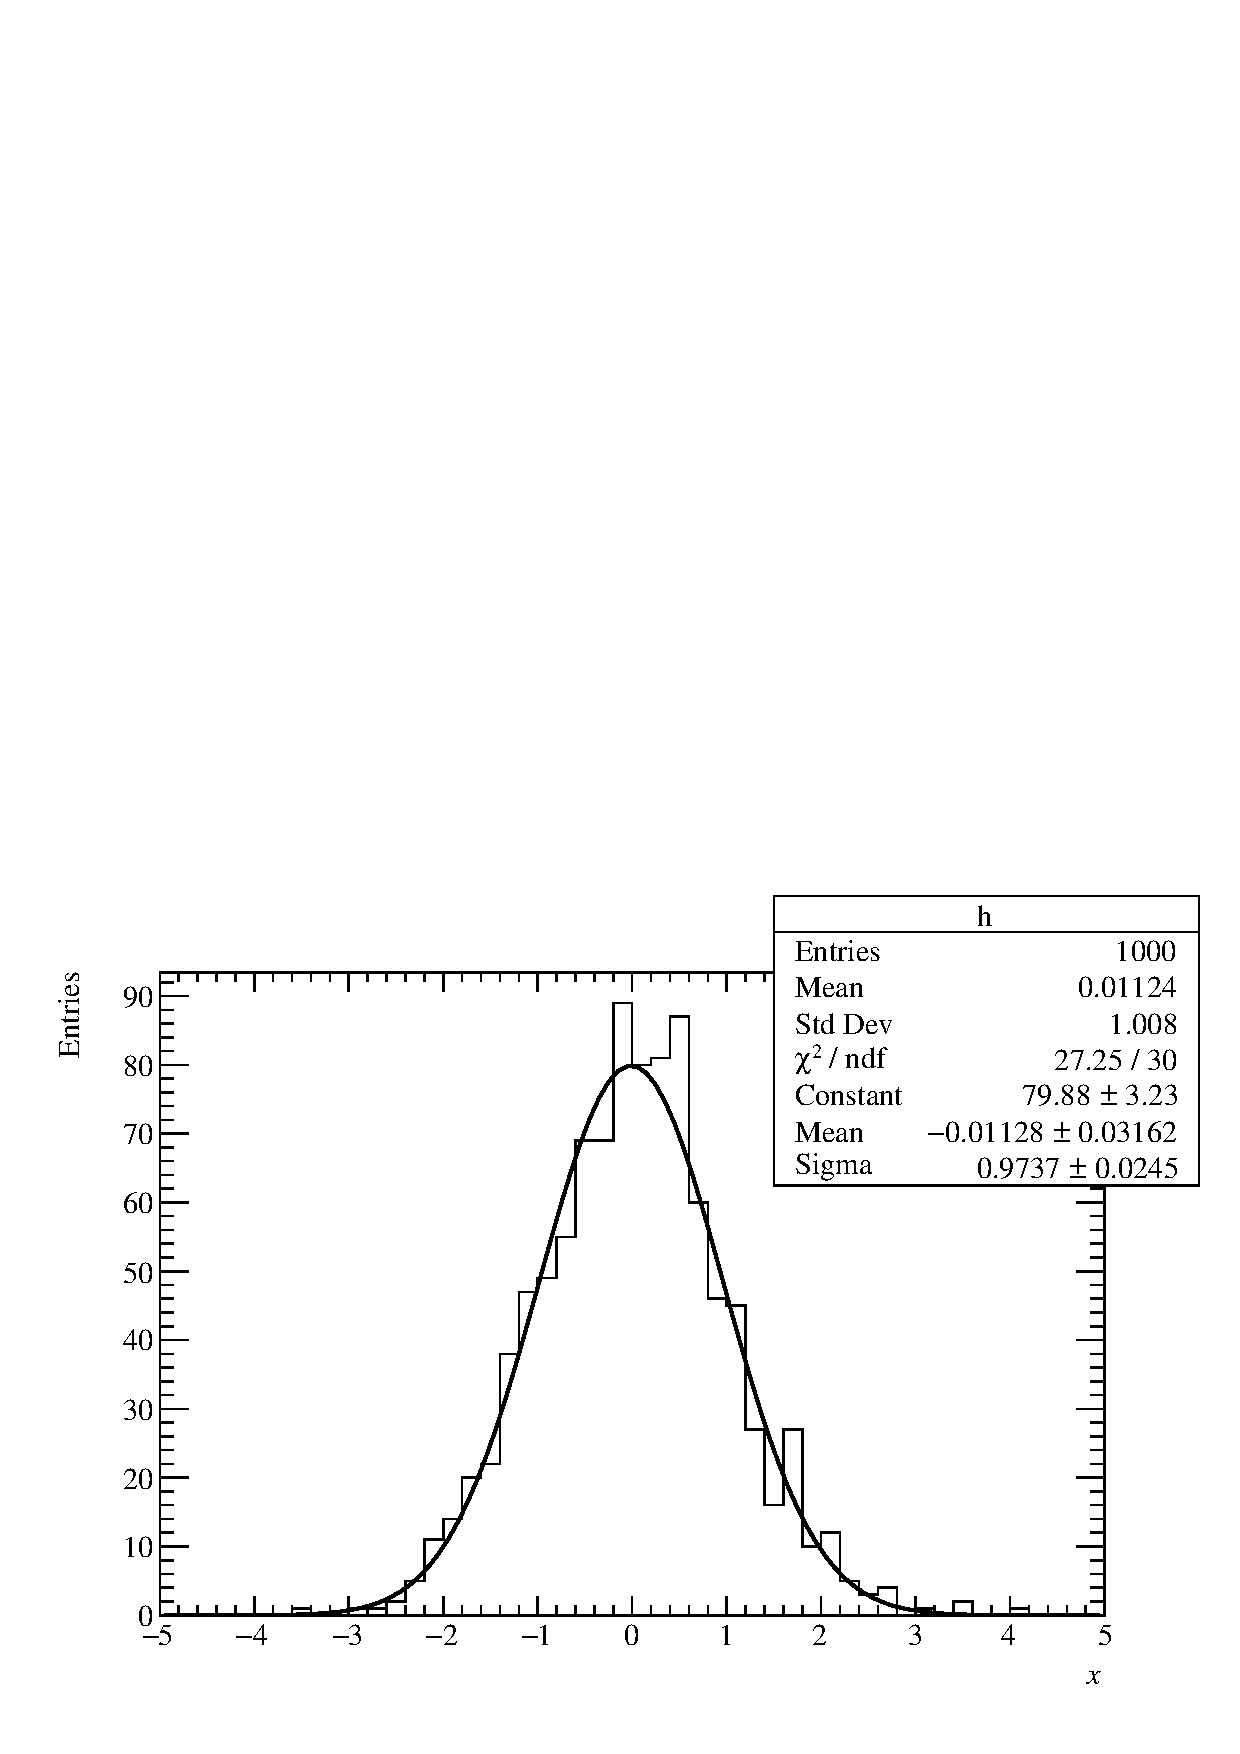
\includegraphics[width=14cm]{fig/histogram.pdf}
  \caption[ガウシアンでヒストグラムをフィットした例]{ガウシアンでヒストグラムをフィットした例。PDF(ベクター画像)なので、出力PDFで拡大しても滑らかです。また文字列もPDF中で検索することができます。}
  \label{fig_histogram}
\end{figure}

図を文中で参照したいときは\texttt{ref}コマンドを使用して、「図~\ref{fig_CTA}」のようにすることができます。この部分は\LaTeX{}中で実際には\texttt{図\~{}\bs{}ref\{fig\_CTA\}}と書いています。「図」と\texttt{\bs{}ref}の間に\texttt{\~{}}を入れるのは、「図」と図番号の間で改行を防ぐためです\footnote{このようにチルダを入れる手法は、人名の姓名の間や数値と単位の間で改行を防ぐのにも広く使われます。}。

\texttt{figure}環境で図を挿入する場所は、初めてその図を言及する段落の直後、もしくは直前です。あまりに離れた場所に図を挿入すると読者はどこに図があるかを探さなくてはならず、読むのが困難になるからです。

場合によっては複数の図を並べたいこともあるでしょう。そのようなときは、\texttt{subfigure}環境を使って図~\ref{fig_subfigure}のようにすることができます。\texttt{minipage}環境でも似たようなことができますが、\texttt{subfigure}を使うと小番号を自動で付与したり、「図~\ref{fig_subfigure_b}」のように、小番号を参照することができます。

\begin{figure}
  \centering
  \subfigure[]{% {の直後に%を置くことで、改行をさせない(図(b)を改行させない)。
    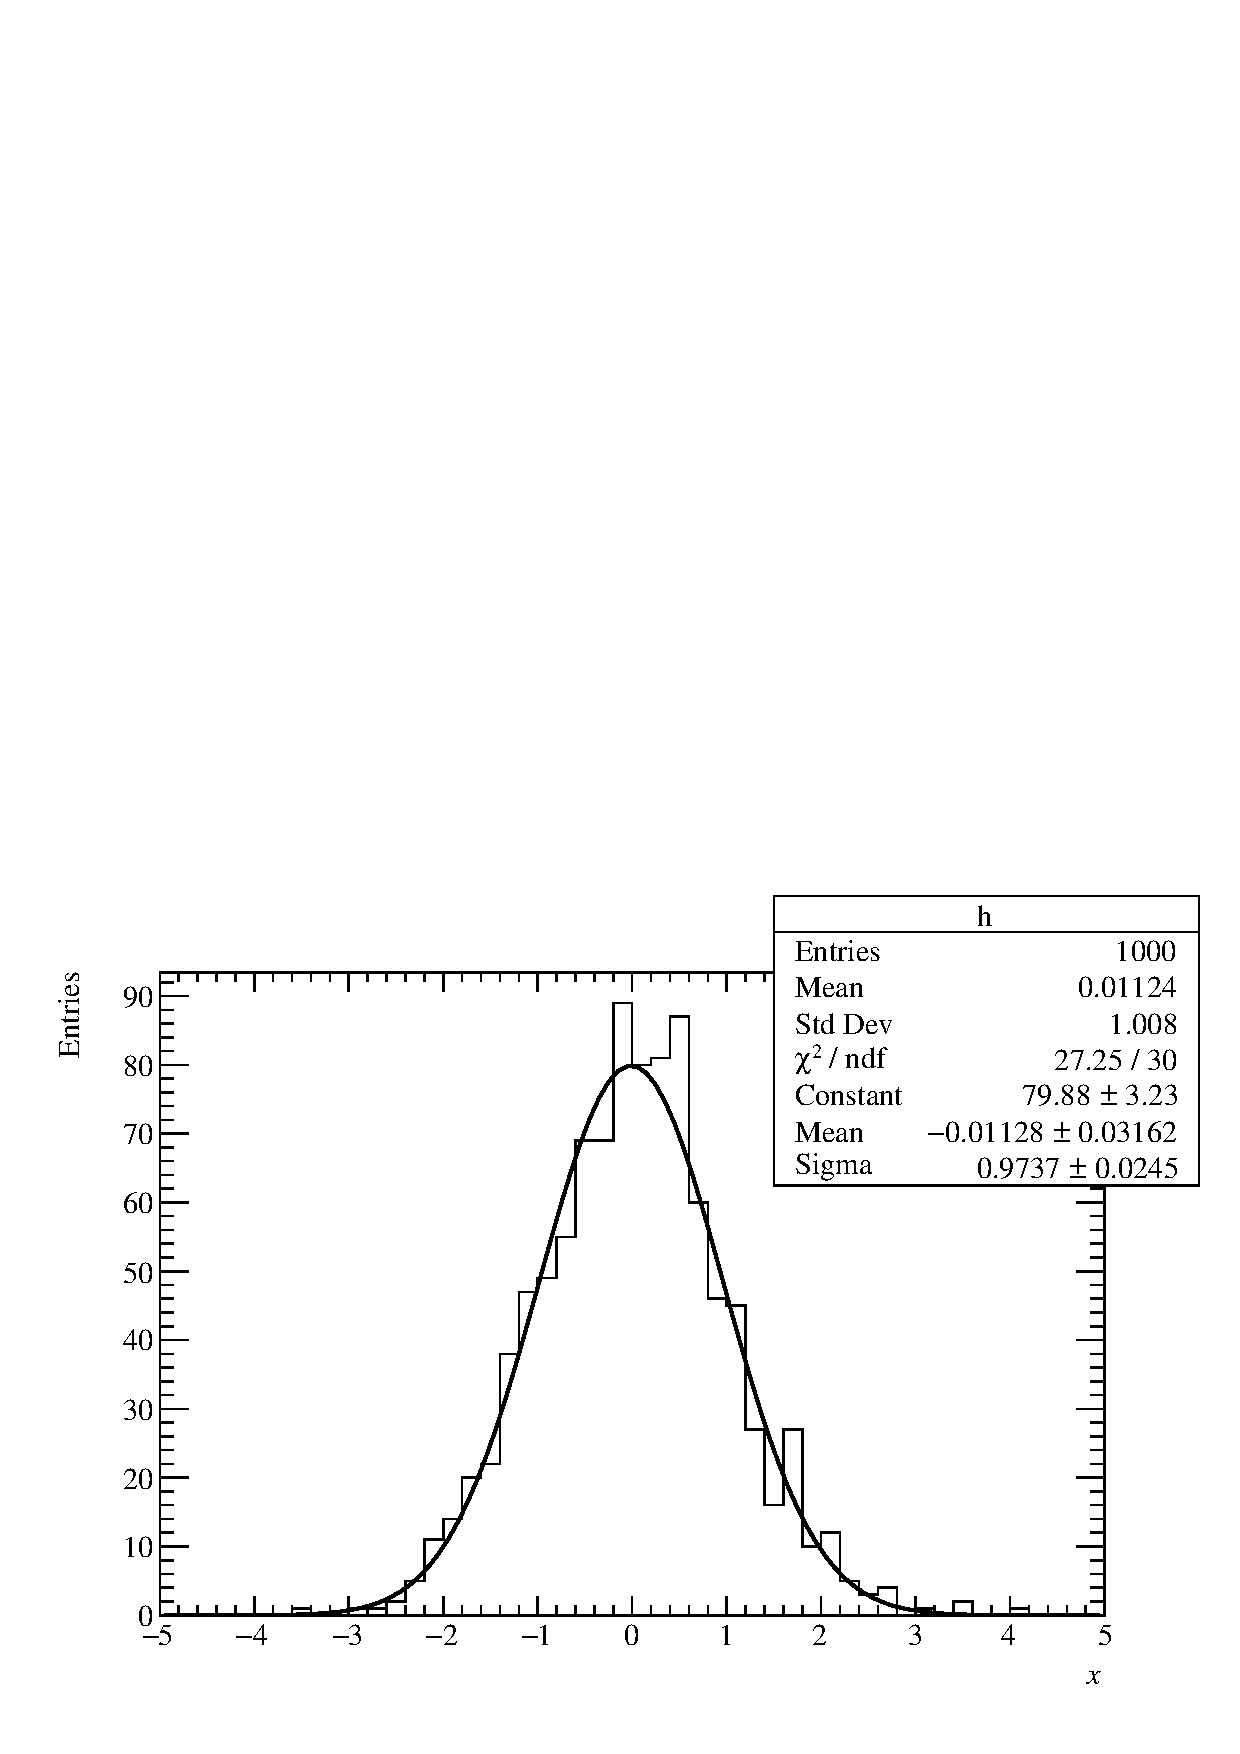
\includegraphics[width=.5\textwidth,clip]{fig/histogram.pdf}%
    \label{fig_subfigure_a}%
  }%
  \subfigure[]{%
    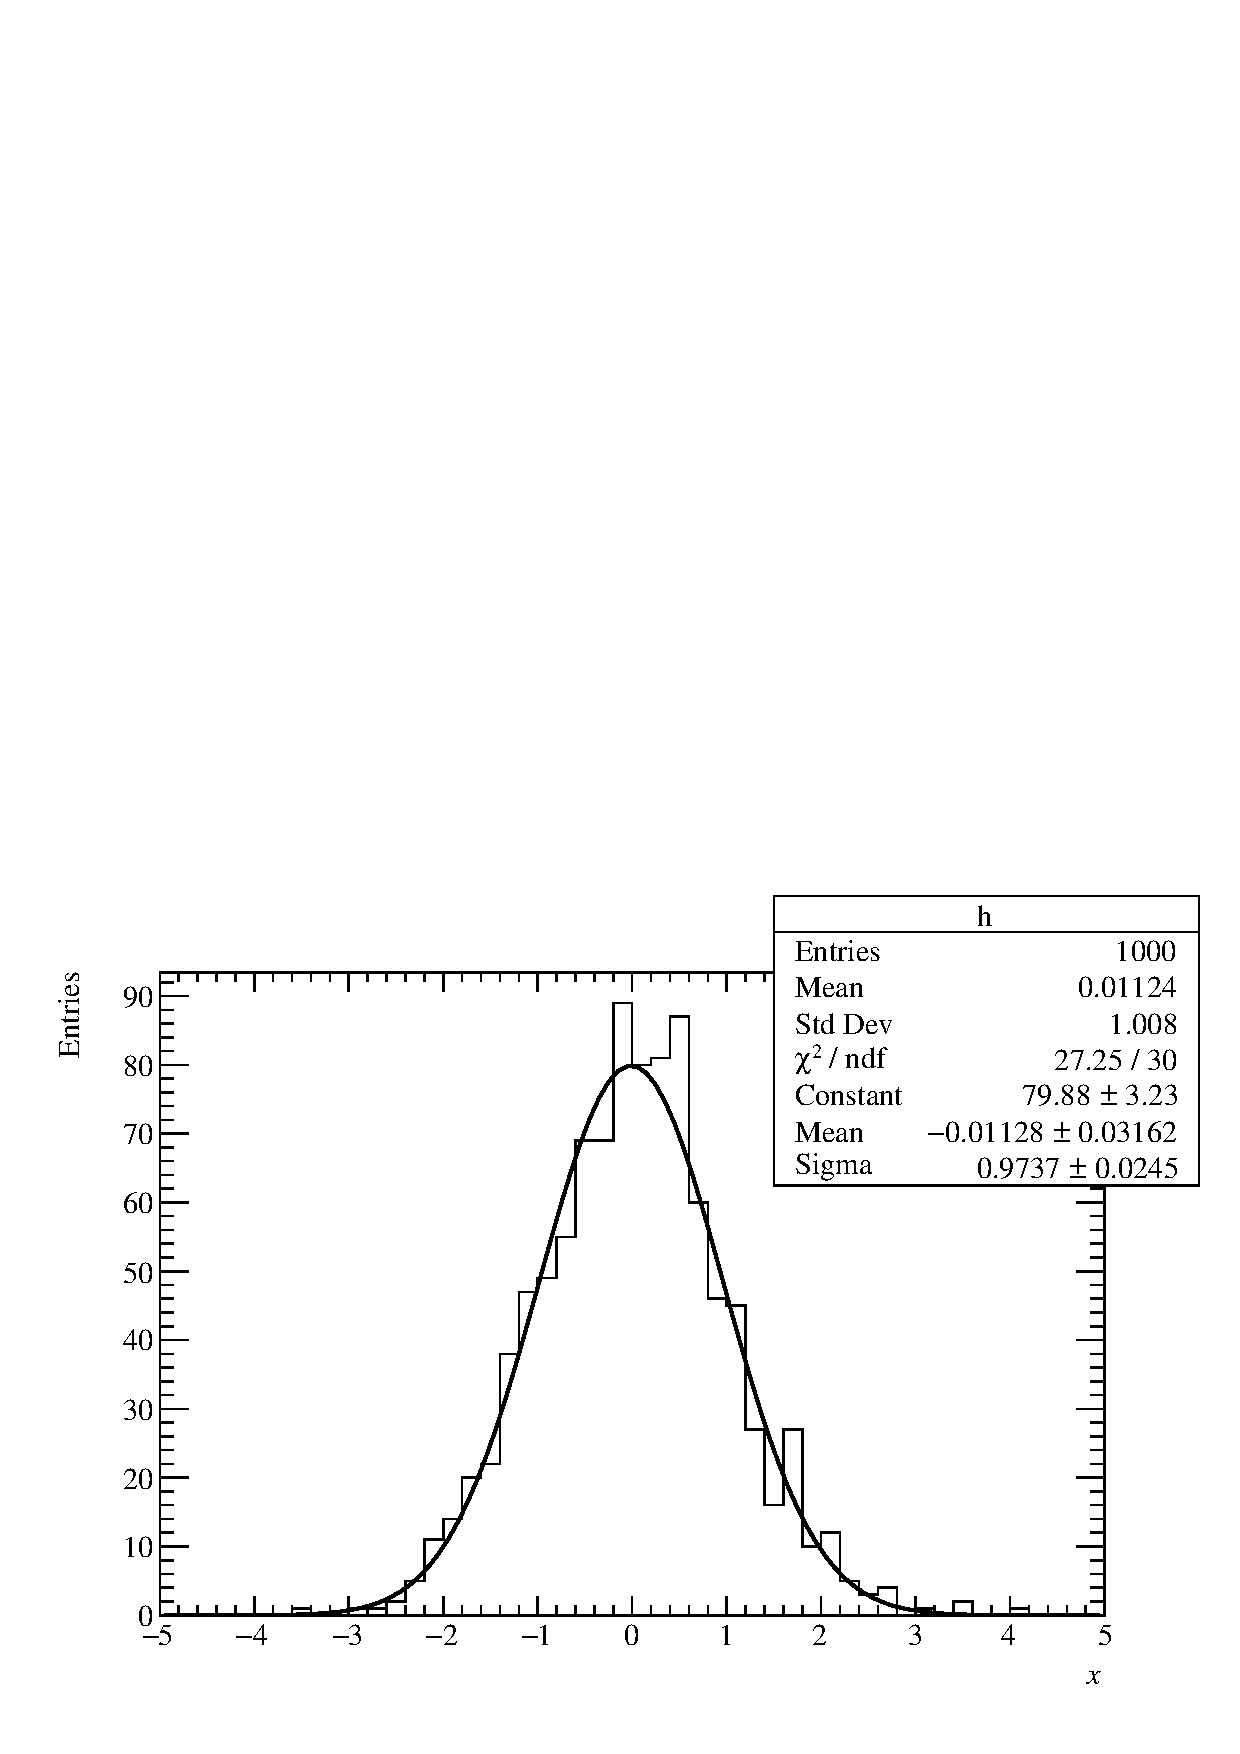
\includegraphics[width=.5\textwidth,clip]{fig/histogram.pdf}%
    \label{fig_subfigure_b}%
  }
  \subfigure[]{%
    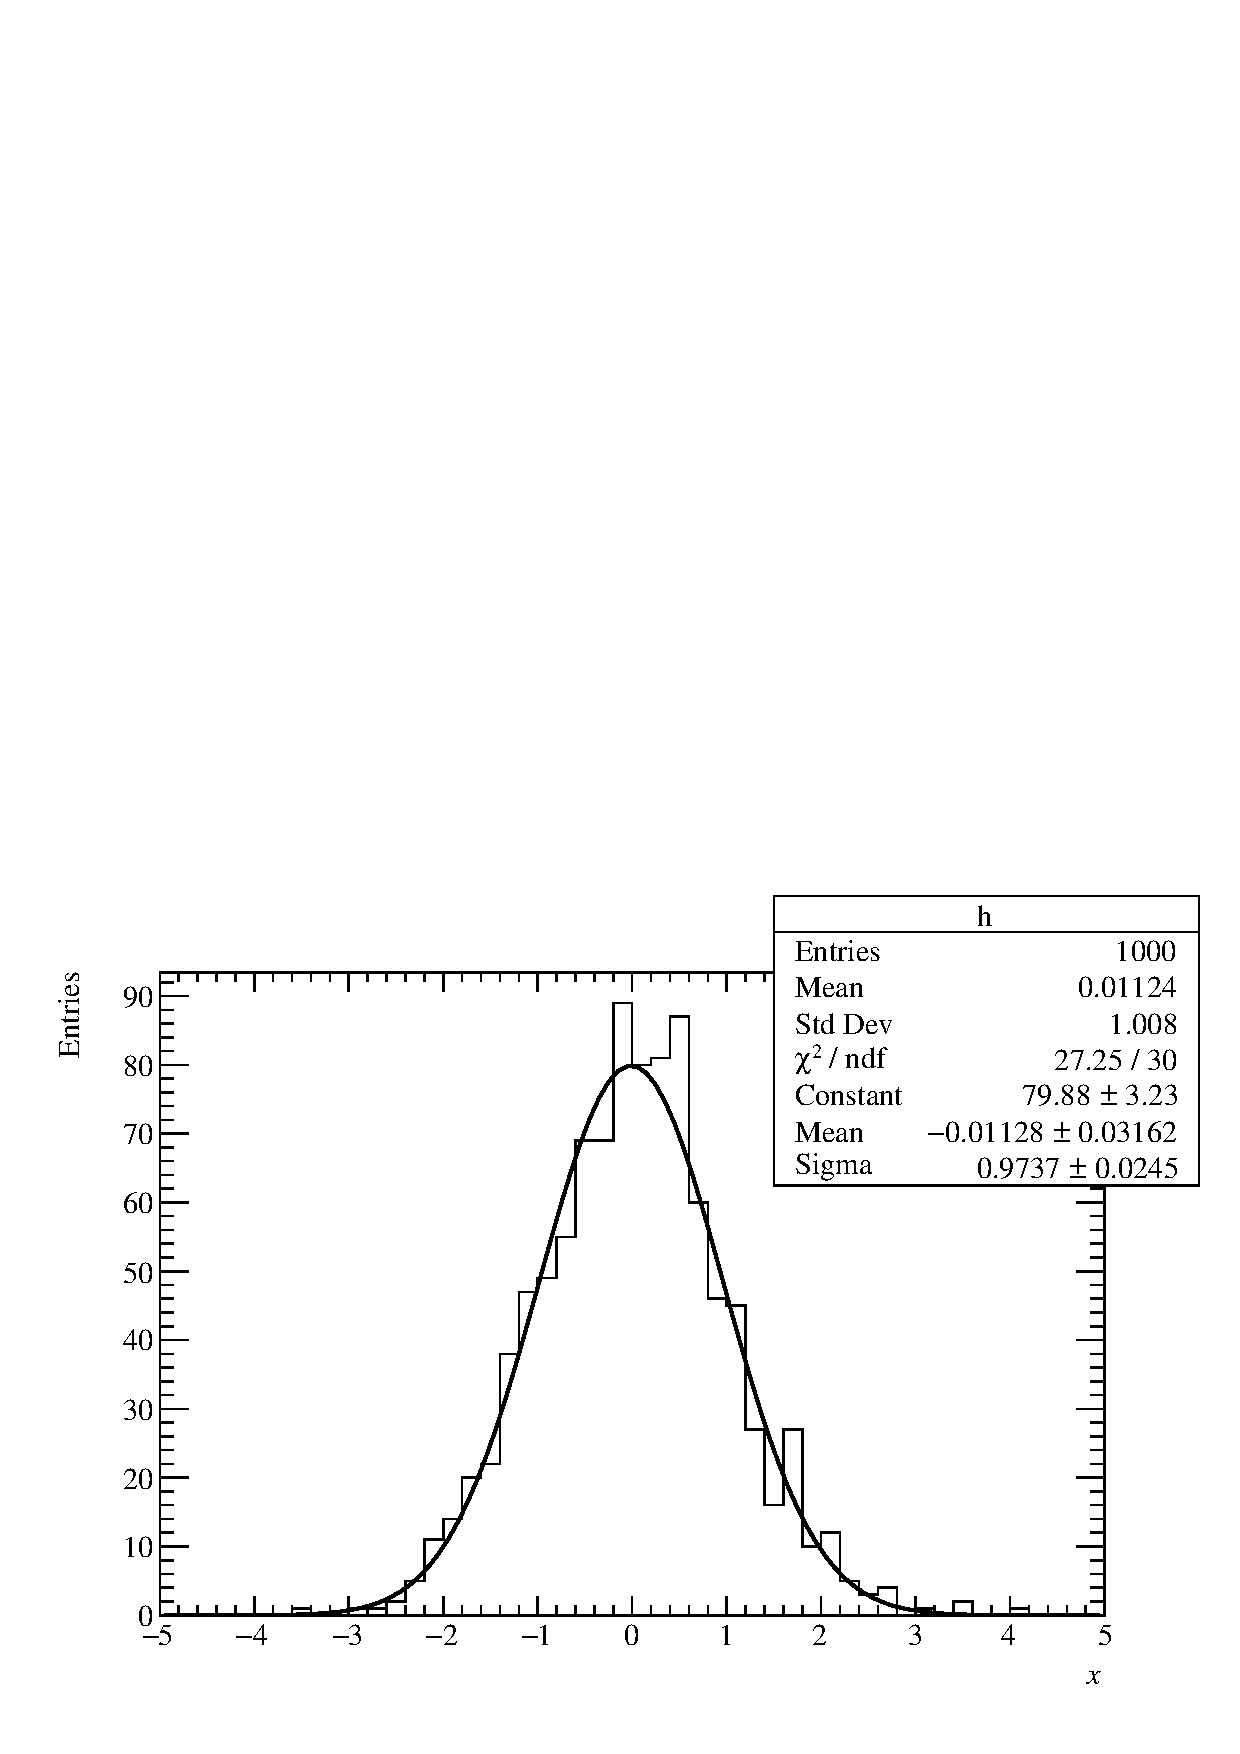
\includegraphics[width=.5\textwidth,clip]{fig/histogram.pdf}%
    \label{fig_subfigure_c}%
  }%
  \subfigure[]{%
    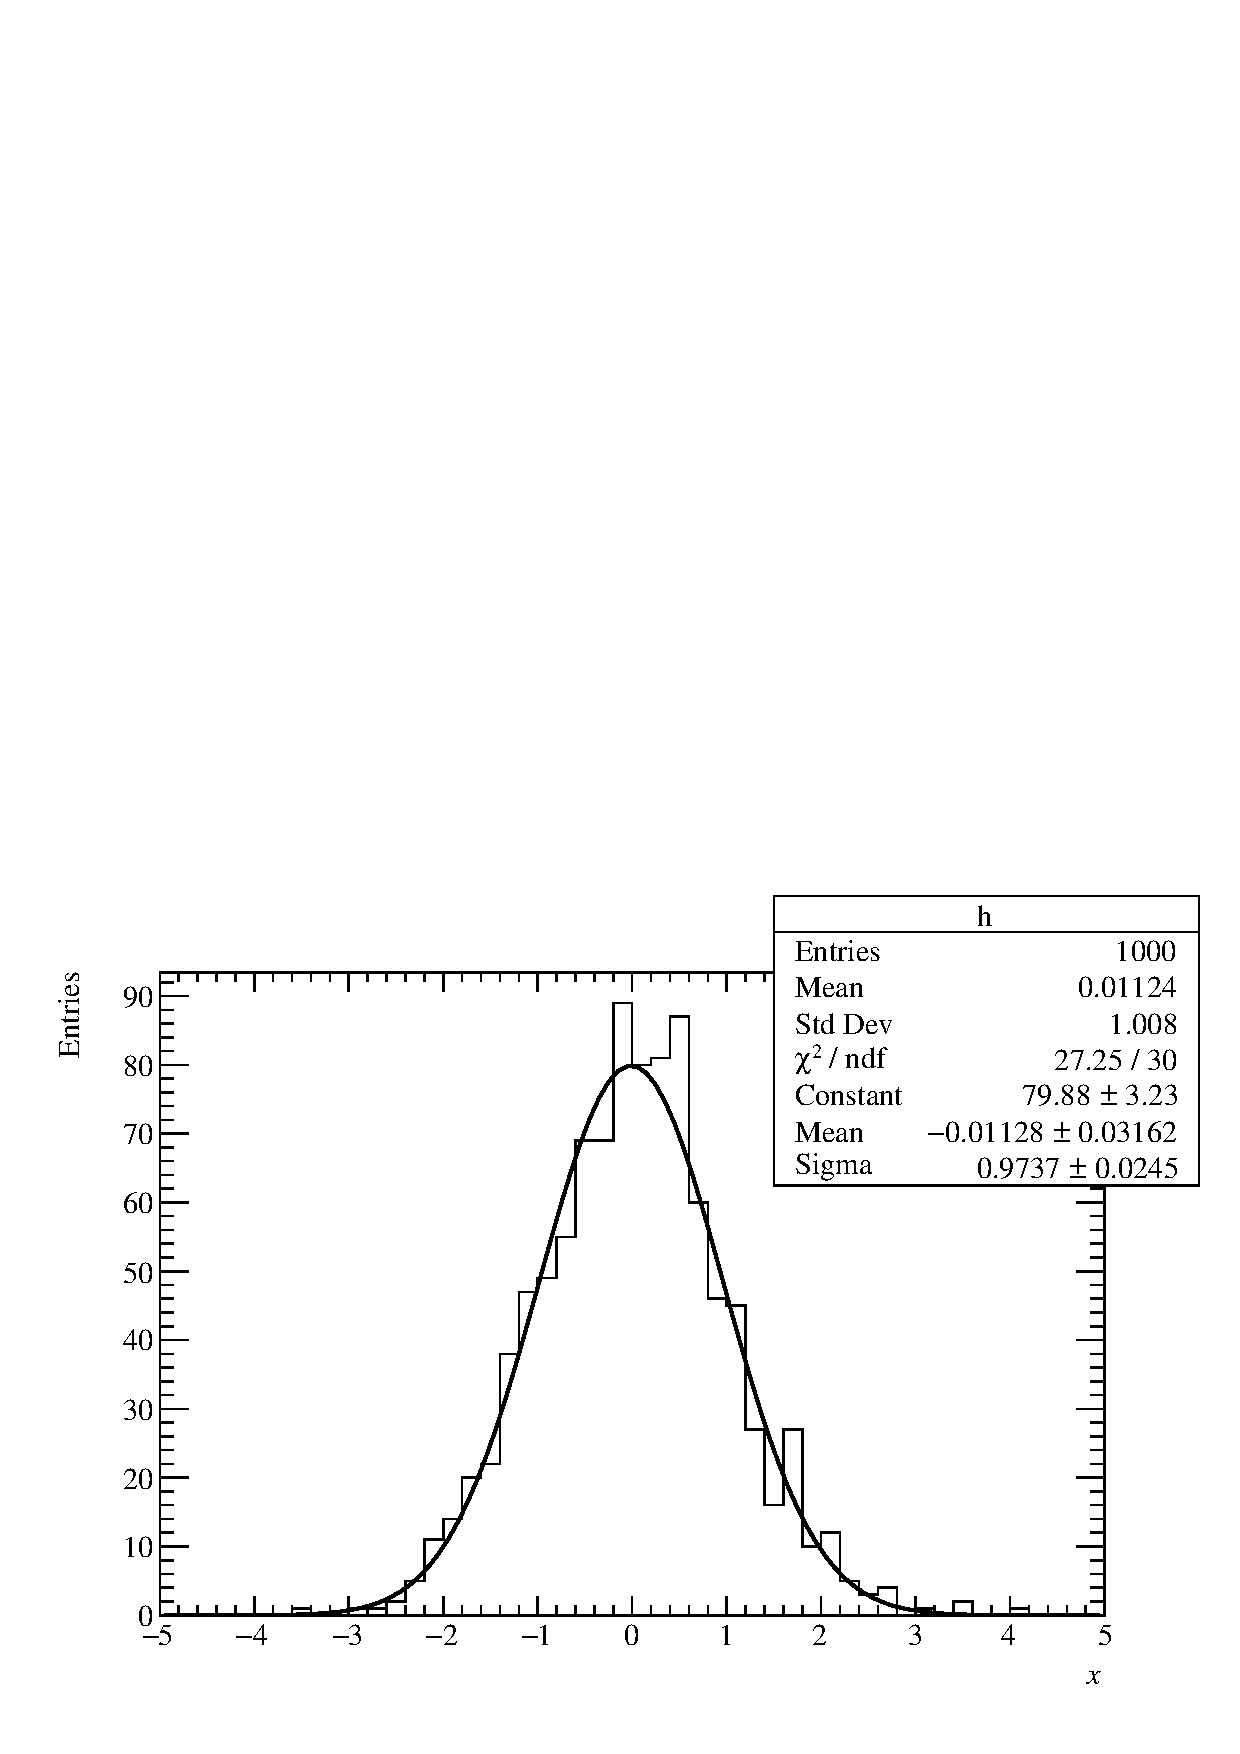
\includegraphics[width=.5\textwidth,clip]{fig/histogram.pdf}%
    \label{fig_subfigure_d}%
  }
  \caption[複数の図を並べた例]{複数の図を並べた例。(a)ガウシアンフィット。(b)同じもの。(c)これも同じもの。(d)これも同じもの。}
\label{fig_subfigure}
\end{figure}

またせっかく図の並べ方が分かったので、同じ図をPDF、PNG、JPEGにして図~\ref{fig_formats}にて比較してみましょう。それぞれの画像の特徴が分かります。また図~\ref{fig_formats}は参考のため\texttt{subfigure}ではなく\texttt{minipage}環境を使って作ってあります。

\begin{figure}
  \begin{minipage}[b]{.3333\linewidth}
    \leftline{(a)}
    \centering
    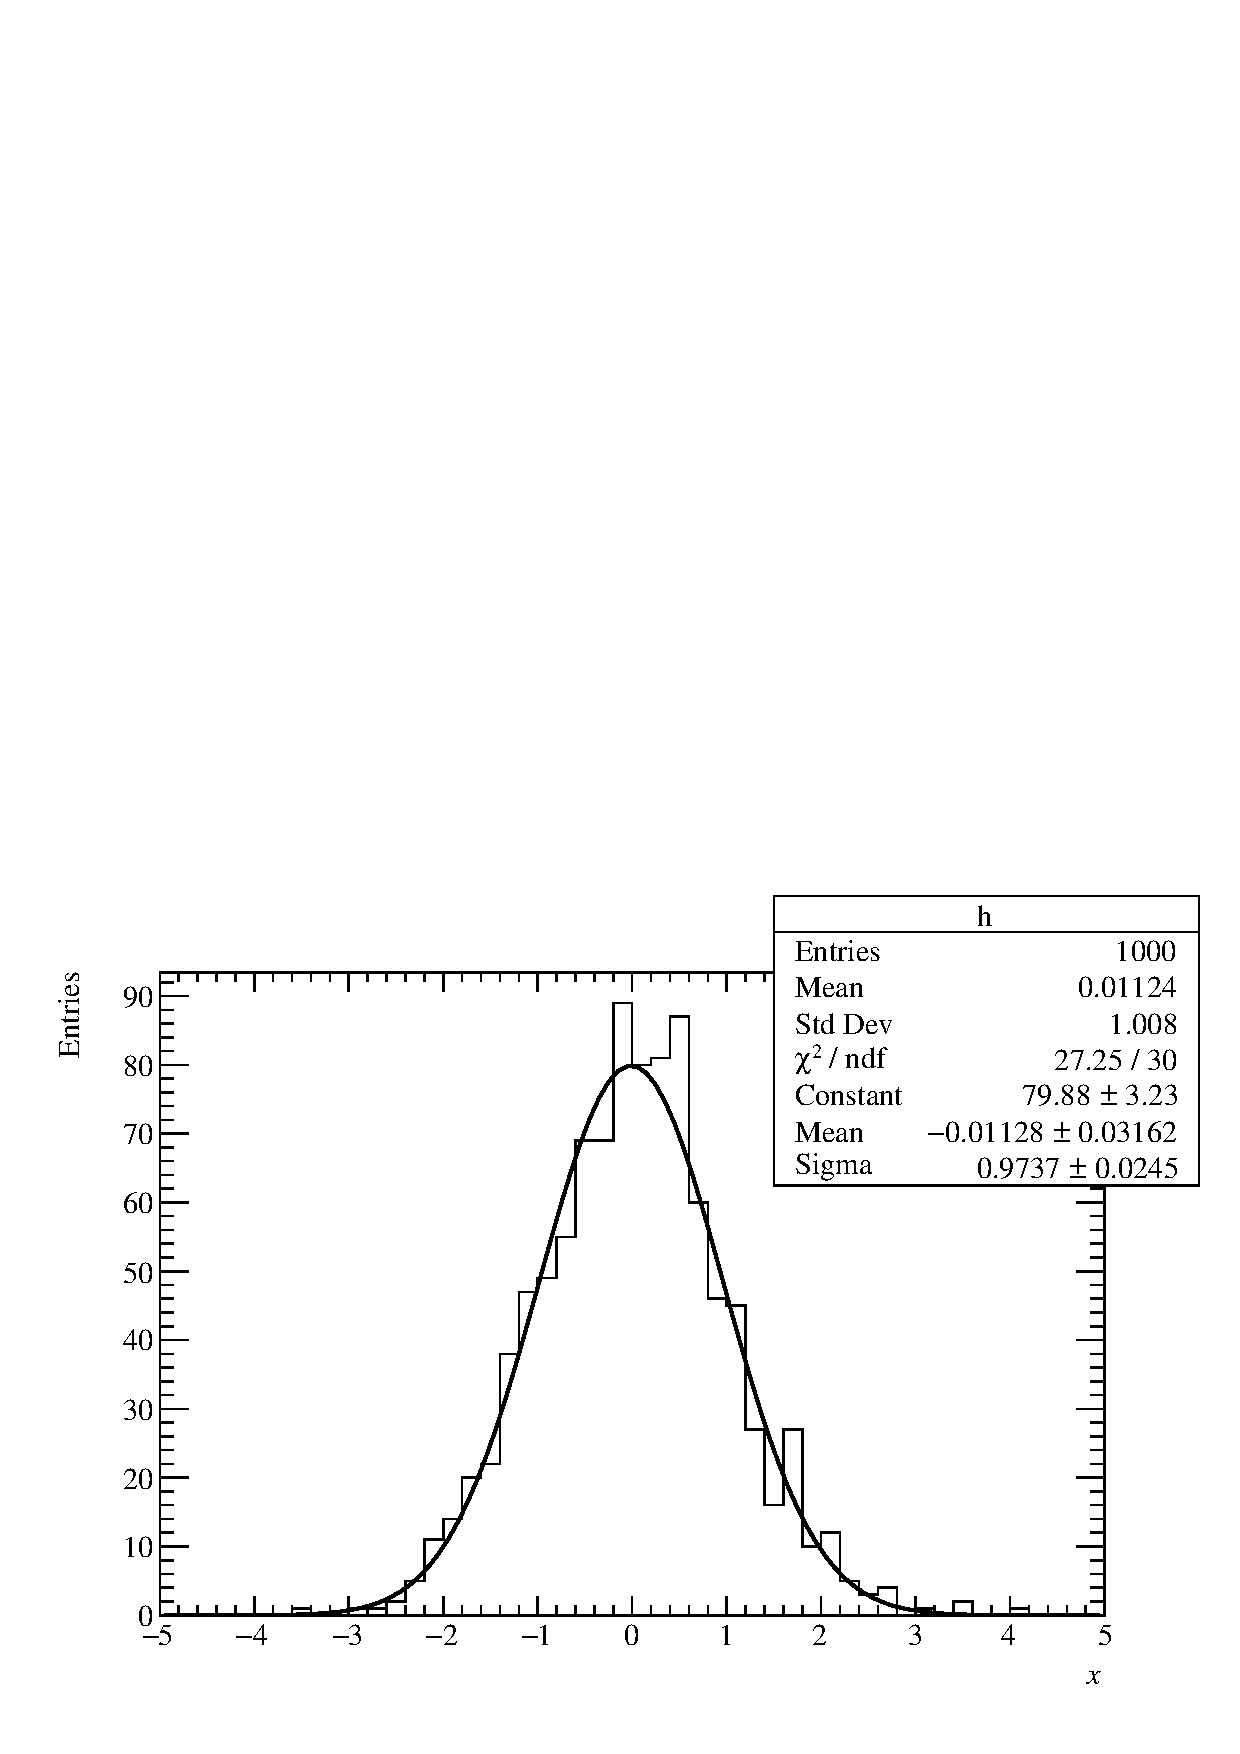
\includegraphics[width=5.5cm]{fig/histogram.pdf}
  \end{minipage}%
  \begin{minipage}[b]{.3333\linewidth}
    \leftline{(b)}
    \centering
    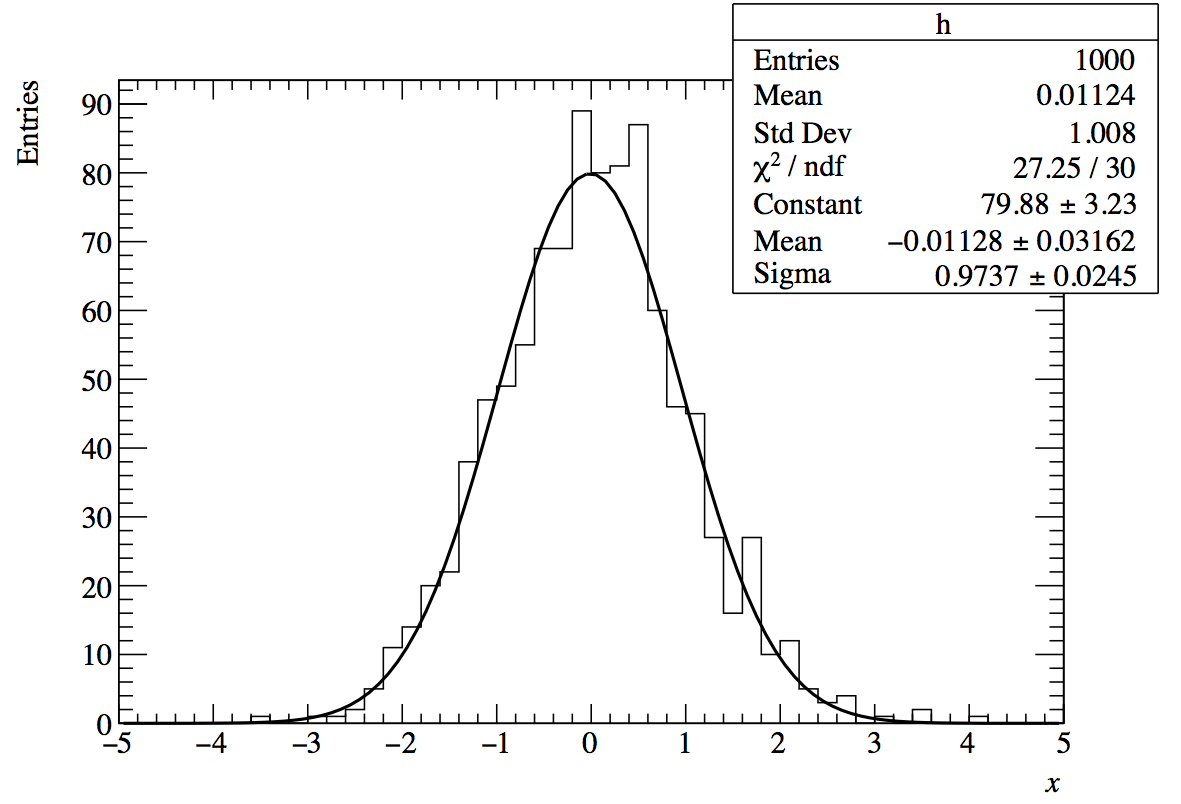
\includegraphics[width=5.5cm]{fig/histogram.png}
  \end{minipage}%
  \begin{minipage}[b]{.3333\linewidth}
    \leftline{(c)}
    \centering
    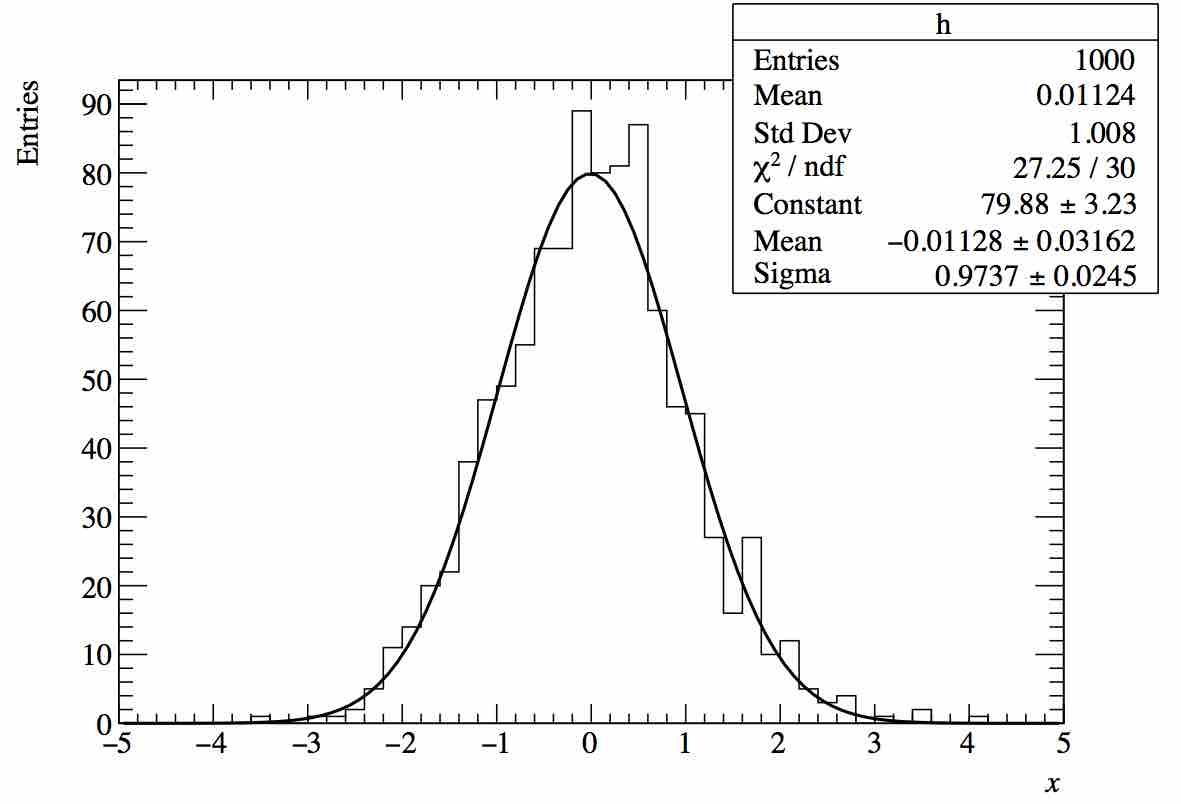
\includegraphics[width=5.5cm]{fig/histogram.jpg}
  \end{minipage}
  \caption[異なる画像形式の比較]{異なる画像形式の比較。(a) PDF形式。拡大しても綺麗であり、文字も検索やコピーができる。(b) PNG形式。拡大するとビットマップ画像であることが分かる。文字を選択できない。(c) JPEG形式。PNGに比べ、JPEG圧縮特有のブロックノイズ、モスキートノイズが発生しており非常に汚いことが分かる。}
  \label{fig_formats}
\end{figure}

\section{表の使い方}

表~\ref{tab_cta}に、\LaTeX{}でどのように表を作成するかの例を示します。実際にどういう \LaTeX{}コードがこの表に対応するのかは、ファイルの中身を眺めてください。

\begin{table} % 表も[htbp]のような場所指定は特に必要ない
  \centering
  % 表のキャプションは必ずその表の上に来ます。図の場合は下です。違いに気をつけてください。
  \caption{CTA で使用される望遠鏡の性能諸元}
  \footnotesize % 横幅のある表なので、文字サイズを小さくしています。通常は必要ありません。
  \label{tab_cta} % ラベルのつけ方は図と同様です。
  \begin{tabular}{lccccccc} % 列が何列あるかを示します。lcrはそれぞれ左・中央・右揃えの指定です。
    \hline
    &
    \shortstack{大口径望遠鏡 \\ Large-Sized Telescope \\ (LST)} &
    % 複数列を結合したいときは、multicolumnを使います。
    \multicolumn{2}{c}{\shortstack{中口径望遠鏡 \\ Medium-Sized Telescope \\ (MST)}} &
    \shortstack{SC 中口径望遠鏡 \\ Schwarzschild--Couder MST \\ (SC-MST)} &
    \multicolumn{3}{c}{\shortstack{小口径望遠鏡 \\ Smalle-Sized Telescope \\ (SST)}} \\
    & & FlashCam & NectarCAM & & GCT & ASTRI & 1M-SST \\
    \hline
    エネルギー範囲 & 20--200 GeV & \multicolumn{2}{c}{100 GeV -- 10 TeV} & 200 GeV -- 10 TeV & \multicolumn{3}{c}{5--300 TeV} \\
台数(北半球)& 4 & \multicolumn{2}{c}{15} & 0 & \multicolumn{3}{c}{0} \\
台数(南半球)& 4 & \multicolumn{2}{c}{24} & 24 & \multicolumn{3}{c}{70--90} \\
鏡直径 &	23~m & \multicolumn{2}{c}{12~m} & 9.7~m & 4~m & 4~m & 4~m \\
焦点距離 & 28~m & \multicolumn{2}{c}{16~m} & 5.6~m & 2.3~m & 2.15~m & 5.6~m \\
視野 & 4.5$^\circ$ & \multicolumn{2}{c}{7.7$^\circ$} & 8$^\circ$ & 8.6$^\circ$ & 9.6$^\circ$ & 9$^\circ$ \\
光学系 & 放物鏡 & \multicolumn{2}{c}{Davies--Cotton (DC)} & Schwarzschild--Couder (SC) & SC & SC & DC \\
画素数 & 1,855 & 1,764 & 1,855 & 11,328 & 2,048 & 1,984 & 1,296\\
\hline
  \end{tabular}
  \normalsize % 文字サイズを元に戻します
\end{table}

論文中で使う表の一般的な注意点として、あまり罫線をたくさん使いすぎないことです。日本では全てのセルの周辺に罫線を使う傾向があり、最悪、表~\ref{tab_cta_bad}のようになります。窮屈になるので、このような罫線の多用はやめましょう。

\begin{table}
  \centering
  \caption{表~\ref{tab_cta}の悪い例}
  \footnotesize
  \label{tab_cta_bad}
  \begin{tabular}{|l|c|cc|c|ccc|}
    \hline
    &
    \shortstack{大口径望遠鏡 \\ Large-Sized Telescope \\ (LST)} &
    % 複数列を結合したいときは、multicolumnを使います。
    \multicolumn{2}{c|}{\shortstack{中口径望遠鏡 \\ Medium-Sized Telescope \\ (MST)}} &
    \shortstack{SC 中口径望遠鏡 \\ Schwarzschild--Couder MST \\ (SC-MST)} &
    \multicolumn{3}{c|}{\shortstack{小口径望遠鏡 \\ Smalle-Sized Telescope \\ (SST)}} \\
    \hline
    & & FlashCam & NectarCAM & & GCT & ASTRI & 1M-SST \\
    \hline
    エネルギー範囲 & 20--200 GeV & \multicolumn{2}{c|}{100 GeV -- 10 TeV} & 200 GeV -- 10 TeV & \multicolumn{3}{c|}{5--300 TeV} \\
    \hline
    台数(北半球)& 4 & \multicolumn{2}{c|}{15} & 0 & \multicolumn{3}{c|}{0} \\
    \hline
    台数(南半球)& 4 & \multicolumn{2}{c|}{24} & 24 & \multicolumn{3}{c|}{70--90} \\
    \hline
    鏡直径 &	23~m & \multicolumn{2}{c|}{12~m} & 9.7~m & 4~m & 4~m & 4~m \\
    \hline
    焦点距離 & 28~m & \multicolumn{2}{c|}{16~m} & 5.6~m & 2.3~m & 2.15~m & 5.6~m \\
    \hline
    視野 & 4.5$^\circ$ & \multicolumn{2}{c|}{7.7$^\circ$} & 8$^\circ$ & 8.6$^\circ$ & 9.6$^\circ$ & 9$^\circ$ \\
    \hline
    光学系 & 放物鏡 & \multicolumn{2}{c|}{Davies--Cotton (DC)} & Schwarzschild--Couder (SC) & SC & SC & DC \\
    \hline
    画素数 & 1,855 & 1,764 & 1,855 & 11,328 & 2,048 & 1,984 & 1,296\\
    \hline
  \end{tabular}
  \normalsize % 文字サイズを元に戻します
\end{table}

\section{数式の使い方}

\LaTeX{}を使う理由のひとつが、数式を綺麗に出力できるというのがあります。例えば中性パイ中間子$\pi^0$のガンマ線への二体崩壊であれば
\begin{equation}
  \pi^0 \rightarrow \gamma + \gamma
\end{equation}
のように書けますし、もっとややこしい数式も色々と書けますが、詳細は「LaTeX 数式」などでインターネット上で検索してください。この例のように、本文中に数式を入れるときは\texttt{\$\$}でその式を囲み、独立した行に数式を書くときは\texttt{equation}や\texttt{align}\footnote{\texttt{amsmath}パッケージで使用可能です。}環境を使ってください。

\subsection{斜体と立体}
数式を書くときには「斜体」(italic)と「立体」(upright)の違いに気をつけてください。基本的に数式は斜体を使って書きます。何も考えずに\LaTeX{}を使えば全て斜体になります。

ただし、次の2つの式を見比べてみてください。
\begin{equation}
  e^{ix}=cosx + isinx
  \label{eq_italic}
\end{equation}
\begin{equation}
  \mathrm{e}^{\mathrm{i}x}=\cos x + \mathrm{i}\sin x
  \label{eq_upright}
\end{equation}
式~\ref{eq_italic}は全ての文字が斜体で書かれていますが、式~\ref{eq_upright}は$x$以外は立体です。このように、いくつかの文字では立体を使うのが一般的です。例えば$\log$、$\sin$、$\mathrm{e}$(自然対数の底)、$\mathrm{i}$(虚数単位)、$\mathrm{d}$(微分作用素)などは、それぞれ\texttt{\bs{}log}、\texttt{\bs{}sin}、\texttt{\bs{}mathrm\{e\}}、\texttt{\bs{}mathrm\{i\}}、\texttt{\bs{}mathrm\{d\}}などと入力することで書くことができます\footnote{自然対数の底や虚数単位の場合は、分野や国によって斜体にするかどうかの違いがあります。また微分作用素は斜体で$d$とする場合もありますが、立体にすることで長さを表すのに頻繁に使われる変数$d$と区別する効果があります。}。

ここで\texttt{\bs{}mathrm}というコマンドが出てきましたが、これは数式中で文字を立体にするためのコマンドです。特定の文字を立体にするときだけでなく、変数名の添字を立体するときにも使います。例えばトリガー回数を示す変数は$N_\mathrm{trigger}$などと書くことがあると思いますが、このときに「trigger」の部分は変数ではありませんので、斜体にしません。

\subsection{単位}
数式中に単位を使うとき、\texttt{\bs{}mathrm}を使わずに$100 MeV$などとしてしまう間違いもよく見られます。このように斜体になったものは変数$M$と$e$と$V$の掛け算であり、単位ではありません。また100MeVのように単位と数値の間にスペースのない書き方をする人も見かけますが、これも間違いです。本文中に書くときは\texttt{100\~{}MeV}とし、\texttt{equation}環境中では\texttt{100\bs{} \bs{}mathrm\{MeV\}}と書きます\footnote{余計なバックスラッシュとスペースは、数字と単位の間にスペースを入れるためです。}。

\LaTeX{}では\texttt{\%}の後ろをコメントとして扱いますので、95\%のようにパーセントの表示をしたい場合には\texttt{95\bs{}\%}のように書きます。\%と数値の間にスペースを入れるかどうかは、流派が2つありますが、私の周りでは入れない人が多いようです\footnote{入れない理由としては、\%は単位ではなく0.01という数だから、というものが挙げられます。}。

\section{引用の仕方}

研究や論文というのは過去に誰かのやった研究を前提として新たに何かを進歩させるためにあります\footnote{「巨人の肩の上に立つ」とよく表現されます。}。しかしあなたの修士論文に全ての過去の研究を書くことはできませんので、引用という形式を使い他の論文をその事実の出典とします。

ここで、「引用」と日本語で書いた場合には「quotation」と「citation」の2つの英語に翻訳され得ますが、我々の論文で通常用いるのは「citation」のほうです。著作権法などで問題になるのは「quotation」のほうなので、間違えないようにしてください。

\LaTeX{}で\texttt{citep}コマンドや\texttt{citet}コマンドを使って論文を引用するときは、例えば次のようになります。

\begin{quote} % ここで LaTeX の体裁を整えるために quote コマンドを使っていますが、ここは「引用」しているわけではりません。
  宇宙線の全粒子スペクトルは図 XX に示すように$10^9$~eVから$10^{20}$~eVまでおよそ$-3$乗の冪で減少している\citep{Swordy2001}。$10^{12}$~eV(1~TeV)付近のガンマ線は超高エネルギーガンマ線と呼ばれ、様々な観測手法が提案されている\citep[例えば][を見よ]{Okumura2005}。この\citet{Okumura2005}の手法では\ldots
% 複数の文献を一度に引用するには \citep{Swordy2001,Okumura2005}とすることもできます。
\end{quote}
ここでは引用を3回していますが、それぞれ\texttt{citep}、\texttt{citep}、\texttt{citet}コマンドを使っています。

このテンプレートの場合、一番後ろに「引用文献」というページがあります。このページを手作業で間違いなく整形するのは面倒です。手でやる代わりに\BibTeX{}という仕組みを使います。\texttt{thesis.bib}というファイルに引用文献の必要な情報が書かれていますので、これを参考にして\BibTeX{}ファイルを作るか、論文をダウンロードするときに\texttt{.bib}ファイルもダウンロードできますので、それを使ってください\footnote{近年は「文献管理ソフト」と呼ばれるものが発達していますので、特に博士進学する学生は好きなものを入れてみてください。}。

\section{ヨーロッパ圏の人名など}
ウムラウトなどの混じったヨーロッパ圏の人名を入力するには、例えばシュレーディンガーの場合、\LaTeX{}では\texttt{Shr\bs{}"\{o\}dinger}と入力することでShr\"{o}dingerと表示すると\LaTeX{}の教科書には書いてあります。しかしいちいちこんなことをするのは面倒ですので、\texttt{main.tex}に書いてある\texttt{\bs{}usepackage[utf8]\{inputenc\}}を使うことで、直接ウムラウトつきの文字を\LaTeX{}のソース中に書いてしまって問題ありません。「ö」と「\"{o}」は、この\LaTeX{}ソース中では違う入力方法で書かれていますが、出力は同一です。

\section{\texttt{newcommand}}

入力が長く、論文中で何度も繰り返し使うような入力はコマンドとして登録することができます。例えば\texttt{\bs{}HI\{\}}や\texttt{\bs{}bs\{\}}といったコマンドを\texttt{main.tex}で定義しており、これらの結果は「\HI{}」や「\bs{}」と表示されます。

\chapter{議論}
ここではこの研究で得られた結果についての議論を行います。測定結果や観測結果などと一緒に議論を進める場合もあるので、必ず必要な章であるとは言えませんが、できる限り研究で得られた事実と自分の議論は分けましょう。

\chapter{結論}
ここには自分の修士論文の結論を書きます。「議論」の章で書かれたことも、再びここに短く書かれます。

「序論」で始めたら「結論」、「はじめに」で始めたら「おわりに」が原則です。ただし、「まとめと今後の展望」などとすることもありますので、好みに応じて変えてください。

\chapter*{付録} % 章番号を出さない
\addcontentsline{toc}{chapter}{付録} % 目次に載せる

「付録」(appendix)は、論文の本文に載せるには情報として邪魔もしくは必須ではないものの、読者にとって有益となるような情報を載せます。付録を必要としない論文ももちろん存在しますので、そこは著者の判断です。

例えば、たくさんの観測データを様々なモデルでフィットした場合、フィット結果の絵がたくさん出てくるはずです。そのような図は本文中に大量に出されても大切な情報を見失ってしまいますので、大部分は付録に載せることが推奨されます。他には、何かしらの長い式変形や証明を載せる必要がある場合、付録に移動する場合があります。

% 付録は chapter の 1 つとして作りますが、章番号は表示しません。
% また付録の 1 つずつはアルファベットで番号付けをするのが一般的です。
\setcounter{section}{0} % section の番号をゼロにリセットする
\renewcommand{\thesection}{\Alph{section}} % 数字ではなくアルファベットで数える
\setcounter{equation}{0} % 式番号を A.1 のようにする
\renewcommand{\theequation}{\Alph{section}.\arabic{equation}}
\setcounter{figure}{0} % 図番号
\renewcommand{\thefigure}{\Alph{section}.\arabic{figure}}
\setcounter{table}{0} % 表番号
\renewcommand{\thetable}{\Alph{section}.\arabic{table}}

\section{すごい長い証明}
式~(\ref{eq})のように、式番号がアルファベットとアラビア数字の組み合わせになるように、\LaTeX{}ソース中で設定してありますので、中身を眺めてみてください。

\begin{equation}
  \label{eq}
  1 + 1 = 2
\end{equation}


\section{すごいたくさんのフィットの図}

\chapter*{謝辞}%
\addcontentsline{toc}{chapter}{謝辞}

「謝辞」(acknowledgments)は、修士論文を作成する上であなたを支えてくれた人への感謝を書く場所です。誰かへの感謝の気持ちを公開の場所で文書にするというのは気恥ずかしいものですし、修士論文以外ではそんなことをした経験がないかもしれませんが、投稿論文では一般的に行われます\footnote{ただし、投稿論文では家族や友人への感謝はあまり書かず、研究費を出した機関や研究の協力をしてくれた研究者などを書くことが多いです。}。

多くの修士論文では指導教員(国立大学の法人化後は、指導教「官」とは言いません)、実験協力してくれた共同研究者、間接的に助言などをくれた研究室の他の教員・先輩・同輩・後輩、研究室の秘書さんなどに謝意を示すことが多いようです。もし奨学金をどこからか受給していたら、奨学金の出所に対しても謝辞を書いても良いでしょう。また家族・恋人・友人に対する感謝も見られますが、恋人の名前は将来隠したくなる場合もあるので注意しましょう。

感謝の気持ちを書く場所ですので、その相手に失礼のないようにしましょう。氏名の漢字の間違いや、職階の間違いが頻繁に見られます。特に助教を助教授と書き間違えたり、准教授を助教授としたりという間違いが目立ちます。



\renewcommand{\bibname}{引用文献} % jecon.bst だと bib の doi を読み込めずエラーを吐くので,ここだけ,削除すること.
\bibliographystyle{jecon}
\bibliography{thesis}

\end{document}
